


\documentclass[12pt]{article}

\setlength{\topmargin}{0pt}
\setlength{\textheight}{9in}
\setlength{\headheight}{0pt}
\setlength{\headsep}{0pt}
\setlength{\oddsidemargin}{0.25in}
\setlength{\textwidth}{6in}
\pagestyle{plain}
\usepackage{amssymb}
\usepackage{graphicx}
\graphicspath{ {./} }

\begin{document}

%\thispagestyle{empty}

%\raisebox{0.6in}[0in]{\makebox[\textwidth][r]{\it
% DRAFT --- a final version will be posted shortly}}
%\vspace{-0.7in}

\begin{center}
\bf\large CS 541: Artificial Intelligence
\end{center}

\noindent
Instructor: Jie Shen
\hfill
Lecture 12               %%% FILL IN LECTURE NUMBER HERE
\\
Scribe:   David Staronka and Omkar Sinha              %%% FILL IN YOUR NAME HERE
\hfill
November 30, 2021                         %%% FILL IN LECTURE DATE HERE

\noindent
\rule{\textwidth}{1pt}

\medskip

%%%%%%%%%%%%%%%%%%%%%%%%%%%%%%%%%%%%%%%%%%%%%%%%%%%%%%%%%%%%%%%%
%% BODY OF SCRIBE NOTES GOES HERE
%%%%%%%%%%%%%%%%%%%%%%%%%%%%%%%%%%%%%%%%%%%%%%%%%%%%%%%%%%%%%%%%

    \section{On Robustness to Adversarial Examples and Polynomial Optimization}
    The empirical success of deep learning has led to numerous unexplained phenomena about which our understanding is limited. The focus of this paper in adversarial robustness, first observed by Sergey et al. On many benchmark datasets, deep neural networks optimized on the training set can be fooled into misclassifying a test example by making a small adversarial perturbation that is imperceptible to humans.
    We study the design of computationally effective algorithms with provable guarantees, that are robust to adversarial(test time) perturbations. While there has been a proliferation of recent work on this, there is still limited theoretic understanding on basic questions like:
    \begin{enumerate}
        \item {When and how can one develop provably robust learning algorithms?}
        \item {What is the price of achieving robustness to adversarial examples in a computationally efficient manner? }
    \end{enumerate}
    The main contribution of this work is to exhibit a strong connection between achieving robustness to adversarial examples and a rich class of polynomial optimization problems, thereby advancing the above questions. In particular, we do the following:
    \begin{enumerate}
        \item {Design computationally efficient robust algorithms  with provable guarantees for a large class of hypothesis, namely linear classifiers and degree-2 polynomial threshold functions(PTFs).}
        \item {Give precise characterization of the price of achieving robustness in a computationally efficient manner for these classes. }
        \item {Design efficient algorithms to certify robustness and generate adversarial attacks in a principled manner for 2-layer neural networks. }
    \end{enumerate}
    \subsection{Adversarial examples}
    While deep learning remains a powerful technique for lot of machine learning problems and can solve them in an efficient manner with high performance, it is found to be vulnerable to adversarial examples. But what are adversarial examples? \\
    
    Lets assume we have a dataset S, and we train a deep learning model W for it such that W works for all the samples in S with high probability. But however an interesting situation arises. Lets take an individual sample(x,y) in the dataset. Now lets take a point very close to it(x',?) ('?' is there as we don't know much about its label right now at this point). We use the model W to classify x', and we find that the label y' for x' is not y. The situation illustrated below.\\
    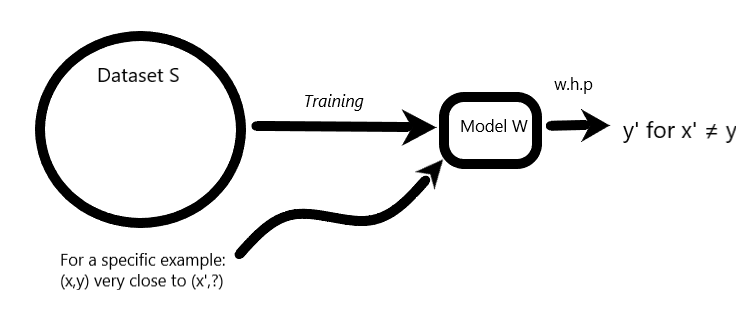
\includegraphics[scale=0.9]{3rd Scribe Notes/Scribe3_1.PNG}
    \\
    Now let's assume that we are classifying this S between dogs and cats. We take an image of a dog(x,y) and very minutely change it(probably a little in brightness or some pixels). As per what we just discussed the model W misclassifies it as cat(x',y'). This is called an adversarial problem as illustrated below.\\
    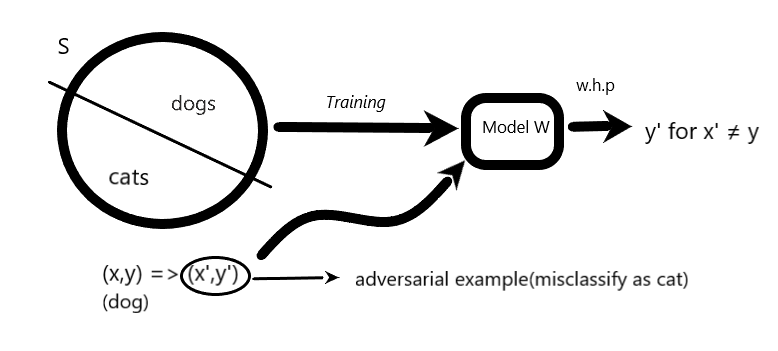
\includegraphics[scale=0.9]{3rd Scribe Notes/Scribe3_2.PNG}
    \\
    \subsection{Polynomial optimization}
    What is polynomial optimization. When we are using polynomial function, in simple language, polynomial optimization is the optimization of polynomial functions.\\
    Lets assume we are training model, we have:\\
    
    $X = {{\{(x_i,y_i)\}}^m_{i=1}}$\\
    
    Since we map every, $x_i$ to $y_i$, we use don't go direct instead using sign function for the transformation:\\
    
    $x_i \rightarrow y_i $ \\
    
    $x_i \rightarrow f(x_i) \rightarrow y_i$ \\
    
    Since, $f(x_i)$ refers to large class of functions and can be real-valued function, we take sign function of it:\\
    
    $x_i \rightarrow f(x_i) \rightarrow sign(f) \rightarrow y_i$ \\
    
    This kind of function is real-valued and d-dimension can be represented as:\\
    
    $f:R^d \rightarrow R $ \\
    
    If we restrict it to polynomial function with domain $(1-,1)$, we get: \\
    
    $h:R^d \rightarrow \{-1,+1\}~~\therefore$ 
    this is Polynomial Threshold function(PTF) \\
    
    Since this is a large class of functions, if we are able to fix the adversarial example problems for this, we have a long way in dealing with this issue.
    \\
    \subsection{Polynomial Threshold Functions(PTFs)}
    In the research paper discussed in this lecture, we establish some methods to find adversarial example using some efficient PTFs.\\
    Lets assume we have trained a model W for dataset S. We would like to verify that this model(W) is robust of all examples,i.e., that every instance in the dataset$(x*,y*)$ there exist no adversarial examples. We use an oracle to predict this as illustrated below:\\
    
    $(x^*\,y^*)\epsilon S, W \rightarrow \framebox[1.1\width]{Oracle} \rightarrow{result} $ \\
    
    Our task is to frame such and efficient 'oracle'. Here we have following input,output and constraints as indicated by above equation: \\
    
    \textbf{input:}\\
    
    $(x^*\,y^*)\,f(PTF)$ \\

    \textbf{output:} 
    \begin{enumerate}
    \item f is robust on $(x^*\,y^*)$
    \item $(x'\,y')$ where f make mistake
    \end{enumerate}
    \textbf{Constraints:}
    \begin{enumerate}
    \item ${\vert \vert\ x^*-x' \vert \vert}_\infty \leq \delta$
    \item $z \epsilon R^d , {\vert \vert\ z ~\vert \vert}_\infty \leq \delta~there~exists~no~x^*\delta~that~is~Adeversarial~example$
    \end{enumerate}
    To find out whether adversarial function exist we maximize the following function: \\
    
    $max~ -sign(f(x^*)).f(x^*+\delta)<0$ where ${\vert \vert\ z ~\vert \vert}_\infty \leq \delta$ \\
    
    In the above formulae z, which is distance between $x^8$ and x' is infinitesimally small. This means that the distinction between original picture and the one put by adversary is not recognizable by human eye.
    \subsection{Optimization of polynomial function}
    It is not always easy to optimize our polynomial function as when the degree become higher is becomes difficult to solve.\\
    
    \textbf{Degree 1 Polynomial Functions}
    Degree 1 basically means linear functions. It can be represented as follows:\\
    
    $f(x)= \sum^n_{i=1}.C_i.x_i$
    \\
    If we want to optimize the linear function its quite easy. All the constraint sets are also linear. To find maximum value in the constraints we only try the maximized values. This can be solved in polynomial time, because its linear time.\\
    
    \textbf{Degree 2 Polynomial Functions}
    With degree 2 polynomial functions the original optimization problem become NP-hard, because there are quadratic terms and cannot be solved in polynomial time. However in machine learning, we always want to solve our problems in polynomial time due to cost factors.
    
     We use the SDP-based algorithm for the degree-2 optimization problem. Its steps are:
    \begin{enumerate}
    \item Given (A, b, c) that defines the polynomial $g(z):=z^TAz+b^Tz+c$
    \item Solve the SDP given by following vector program: \\
    $max~\sum_{i,j}A_{i,j}<u_i,u_j>+\sum_i b_i <u_i,u_0>+c~subject~to~ {\vert \vert\ u\vert \vert\ }_2^2\leq \delta^2~\forall i \epsilon [n]\,~{\vert \vert\ u\vert \vert\ }^2_2=1 $
    \item Let $u_i^\bot$ represent the component of $u_i$ orthogonal to $u_0$. Draw $S \geq N(0, I)$ a standard Gaussian vector, and set $\hat{z_i}:=<u_i,u_0>+<u_i^\bot,S>$ for each $i \epsilon\{0,1,..n\}$
    \item Repeat rounding $O(\log(1/n))$ random choices of S and pick the best choice.
    \end{enumerate}
     
    \section{From Adversarial Examples to Robust Learning Algorithms}
    In this section, we leverage the algorithms for finding adversarial examples to design polynomial time robust learning algorithms for various sub-classes of Polynomial Threshold Functions(PTF). These include general degree-1 and degree-2 PTFs. We obtain our upper bounds bu establishing a general algorithmic framework that relates robust learnability of PTFs to the polynomial maximization problem from the previous section, defined as:
    
    \subsection{$\gamma$-factor admissibility}
    for $\gamma\ge1$, we say that a sub-class $\mathcal{F}$ of PTFs is $\gamma$-factor admissable if $\mathcal{F}$ has the following properties:
    \begin{enumerate}
        \item for any $a, b, c \in \mathbb{R}, sgn(f(x)), sgn(g(x))\in\mathcal{F}, sgn(af(x)+bg(x)+c)\in\mathcal{F}$
        \item for any $b\in\mathbb{R}^n$ and $sgn(g(x))\in\mathcal{F}$, we have that $sgn(g(x+b))\in\mathcal{F}$
        \item there is a $\gamma$-admissable approximation for $\{g:sgn(g)\in\mathcal{F}\}$
    \end{enumerate}
    
    As long as $\mathcal{F}$ meets these conditions, we can define a new algorithm to train a robust classifier in $\mathcal{F}$ defined as:
    \begin{enumerate}
        \item Let $S=(x_1,y_1), (x_2,y_2),...,(x_m,y_m)$ be the given training set
        \item Find a degree polynomial $g\in\mathcal{F}$ that satisfies: \\ 
        $y_{i}g(x_i)>r_i,\forall i\in [m]$ \\
        $r_i\ge$ \(\sup\limits_{z \in B^{n}_{\infty}(0, \delta)}\) $y_{i}(g(x_{i})-g(x_{i}+z)),\forall i\in [m]$
    \end{enumerate}
    For any g that satisfies the above, that g is said to be robust
    %%%%%%%%%%%%%%%%%%%%%%%%%%%%%%%%%%%%%%%%%%%%%%%%%%%%%%%%%%%%%%%%

\end{document}